\documentclass{article}
\usepackage{latexmldoc}
\newcommand{\LTXLaTeXML}{\pkg{LaTeXML}}
\newcommand{\LTXObject}{\pkg{LaTeXML::Object}}
\newcommand{\LTXState}{\pkg{LaTeXML::State}}
\newcommand{\LTXToken}{\pkg{LaTeXML::Token}}
\newcommand{\LTXTokens}{\pkg[LaTeXML::Token]{LaTeXML::Tokens}}
\newcommand{\LTXNumber}{\pkg[LaTeXML::Token]{LaTeXML::Number}}
\newcommand{\LTXDimension}{\pkg[LaTeXML::Token]{LaTeXML::Dimension}}
\newcommand{\LTXMuDimension}{\pkg[LaTeXML::Token]{LaTeXML::MuDimension}}
\newcommand{\LTXGlue}{\pkg[LaTeXML::Token]{LaTeXML::Glue}}
\newcommand{\LTXMuGlue}{\pkg[LaTeXML::Token]{LaTeXML::MuGlue}}
\newcommand{\LTXBox}{\pkg{LaTeXML::Box}}
\newcommand{\LTXMathBox}{\pkg[LaTeXML::Box]{LaTeXML::MathBox}}
\newcommand{\LTXComment}{\pkg[LaTeXML::Box]{LaTeXML::Comment}}
\newcommand{\LTXList}{\pkg[LaTeXML::Box]{LaTeXML::List}}
\newcommand{\LTXMathList}{\pkg[LaTeXML::Box]{LaTeXML::MathList}}
\newcommand{\LTXWhatsit}{\pkg[LaTeXML::Box]{LaTeXML::Whatsit}}
\newcommand{\LTXFont}{\pkg{LaTeXML::Font}}
\newcommand{\LTXMathFont}{\pkg[LaTeXML::Font]{LaTeXML::MathFont}}
\newcommand{\LTXDocument}{\pkg{LaTeXML::Document}}
\newcommand{\LTXDefinition}{\pkg{LaTeXML::Definition}}
\newcommand{\LTXExpandable}{\pkg[LaTeXML::Definition]{LaTeXML::Expandable}}
\newcommand{\LTXPrimitive}{\pkg[LaTeXML::Definition]{LaTeXML::Primitive}}
\newcommand{\LTXRegister}{\pkg[LaTeXML::Definition]{LaTeXML::Register}}
\newcommand{\LTXConstructor}{\pkg[LaTeXML::Definition]{LaTeXML::Constructor}}
\newcommand{\LTXParameters}{\pkg{LaTeXML::Parameters}}
\newcommand{\LTXParameter}{\pkg[LaTeXML::Parameter]{LaTeXML::Parameter}}
\newcommand{\LTXKeyVals}{\pkg[LaTeXML::Parameter]{LaTeXML::KeyVals}}
\newcommand{\LTXMouth}{\pkg{LaTeXML::Mouth}}
\newcommand{\LTXFileMouth}{\pkg[LaTeXML::Mouth]{LaTeXML::FileMouth}}
\newcommand{\LTXStyleMouth}{\pkg[LaTeXML::Mouth]{LaTeXML::StyleMouth}}
\newcommand{\LTXPerlMouth}{\pkg[LaTeXML::Mouth]{LaTeXML::PerlMouth}}
\newcommand{\LTXGullet}{\pkg{LaTeXML::Gullet}}
\newcommand{\LTXStomach}{\pkg{LaTeXML::Stomach}}
\newcommand{\LTXIntestine}{\pkg{LaTeXML::Intestine}}
\newcommand{\LTXModel}{\pkg{LaTeXML::Model}}
\newcommand{\LTXRewrite}{\pkg{LaTeXML::Rewrite}}
\newcommand{\LTXMathParser}{\pkg{LaTeXML::MathParser}}

\title{\LaTeXML: a \LaTeX\ to \XML\ Converter; \\
       \emph{Preview Version 0.3.0}}
\author{Bruce R.~Miller}
\begin{document}
\maketitle
\section{Introduction}
For many, \LaTeX\ is the prefered format for document authoring, particularly when
significant mathematical content and quality typesetting is involved.
On the other hand, content-oriented \XML\ is an extremely useful representation for documents,
allowing them to be used, and reused, for a variety of purposes, not least, 
presentation on the Web.  Both of these representations were natural and uncontroversial
choices for the corresponding phases of
the \URL[Digital Library of Mathematical Functions]{http://dlmf.nist.gov}.
Yet, the style and intent of \LaTeX\ markup, as compared to \XML\
markup, presents difficulties in converting from the former to the latter.
Perhaps ironically, these difficulties are worst for mathematical material, where
there is a tendency with \LaTeX\ to focus on appearance rather than meaning.
Faced with the need to perform this conversion and the lack of suitable tools to perform it, 
the DLMF project proceeded to develop thier own tool, \LaTeXML, for this purpose.
This document describes a \emph{preview} release of \LaTeXML.

The idealistic goals of \LaTeXML\ are:
\begin{itemize}
\item Faithful emulation of \TeX's behaviour.
\item Easily extensible.
\item Lossless; preserving both semantic and presentation cues.
\item Uses abstract \LaTeX-like, extensible, document type.
\item Determine the semantics of mathematical content\\
    (Content \MathML, \emph{Good} Presentation \MathML, eventually \OpenMath).
\end{itemize}

As these goals are not entirely practical, or even somewhat contradictory,
they are implicitly modified by ``as much as possible.''
Completely mimicing \TeX's behaviour would seem to require the sneakiest modifications
to \TeX, itself.  `Ease of use,' of course, is in the eye of the beholder.
More significantly, few documents are likely to have completely unambiguous
mathematics markup; human understanding of both the topic and the surrounding 
text is needed to properly interpret any particular fragment.
Thus, rather than pretend to provide a `turn-key' solution,
we expect that document-specific declarations or tuning to be necessary
to faithfully convert documents.  Towards this end, we provide a variety
of means to customize the processing and declare the author's intent.
At the same time, especially for new documents, we encourage a more logical, 
content-oriented markup style, over a purely presentation-oriented style.

\medskip
This document continues with an overview of the usage of \LaTeXML (\S\ref{sec:usage})
and its architecture (\S\ref{sec:architecture}).   
In \S\ref{sec:packages}, an overview of customizing \LaTeXML\ is given.
How mathematics is converted to content-oriented forms is discussed in \S\ref{sec:math}.
Finally, Appendix \ref{app:hierarchy} shows an object hierarchy of the system
and Appendix \ref{app:todo} lists the main problem areas and unfinished features.

In general, for more detail, you should see the perl documentation of various
\LaTeXML\ Packages (using, for example, the command \texttt{perldoc LaTeXML}),
or the source code itself, and the examples.

\section{Using \LaTeXML}\label{sec:usage}
The basic conversion to \XML\ (using the \LaTeXML\ DTD, by default) is carried out
by the command:
\begin{quote}
 \cmd{latexml \textit{options} document.tex > document.xml}
\end{quote}
This command reads and processes the \TeX\ document \texttt{document.tex},
along with any document-specific customization (see \S\ref{sec:packages})
in \texttt{document.latexml}, if present,
and constructs an \XML\ document from it.  The document tree is then subjected to various 
rewriting before being passed to the mathematics parser.  The parser applies a grammar based
recursive descent parser to the mathematical content in an attempt to convert
to semantic forms.  (Or, at least to structure consistent with the semantics).

Additional transformations, such as to \HTML, \MathML\ or other formats, are carried out
by stylesheets or postprocessing modules in the postprocessor \cmd{latexmlpost}:
\begin{quote}
\cmd{latexmlpost \textit{options} document.xml}
\end{quote}

See the documentation for the commands \pkg{latexml} and \pkg{latexmlpost} for details
and description of command options\footnote{Use \texttt{latexml --help} or 
\texttt{perldoc latexml} to view the documentation}.

\section{Architectural Overview}\label{sec:architecture}
Like \TeX, \LaTeXML\ is data-driven: the text and control sequences (ie.~macros and primitives)
in the source file (and any packages loaded) direct the processing.
The user exerts control over the processing, and customizes it, by 
providing alternative \LaTeXML-specific implementations of the control sequences and packages,
by declaring properties of the desired document structure,
and by defining rewrite rules to be applied to the constructed document tree.

\begin{figure}[tb]
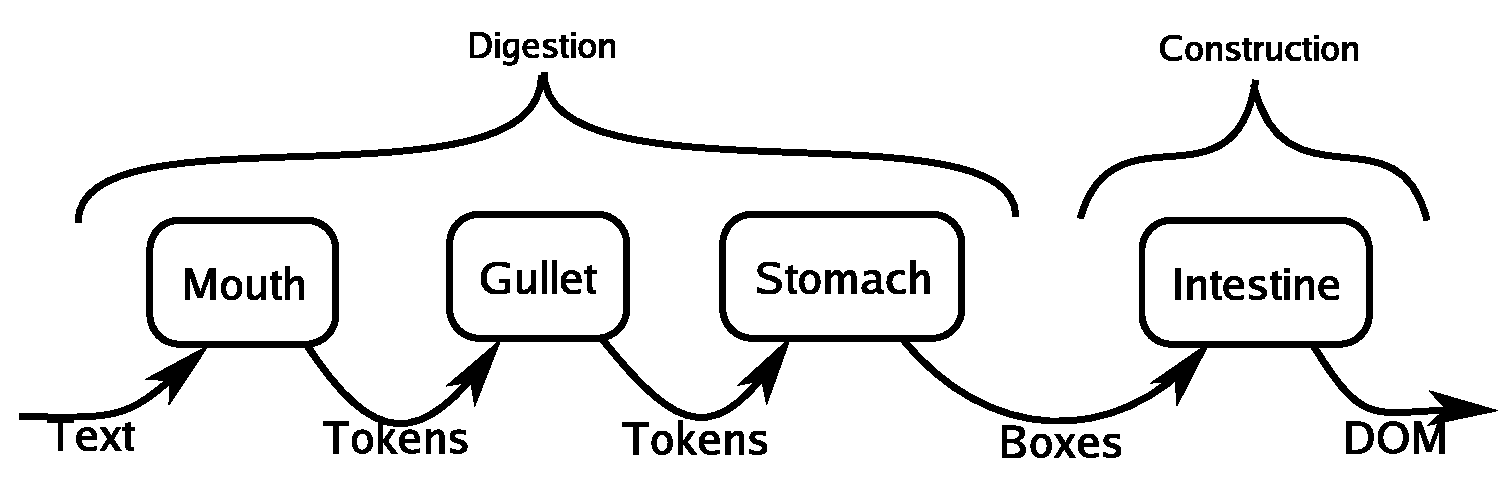
\includegraphics[width=\columnwidth]{dataflow}
\caption{Flow of data through \LaTeXML's digestive tract.\label{fig:dataflow}}
\end{figure}
The top-level class, \LTXLaTeXML, manages the processing, providing several methods
for converting a \TeX\ document or string into an \XML\ document, with varying degrees
of postprocessing and optionally writing the document to file.
A \LTXState\ object maintains the current state
of processing, current definitions for control sequences and emulates the
\TeX's scoping rules.
The processing is broken into two phases; the \TeX-like digestion phase and
the \XML\ construction phase; See Figure \ref{fig:dataflow}.

\emph{Digestion} is carried out primarily in a \emph{pull} mode, with the \LTXStomach\
pulling expanded  \LTXToken's from a \LTXGullet, which, itself pulls tokens from 
a \LTXMouth.  The \LTXMouth\ converts characters from the plain text input into tokens according
to the current category codes assigned to them (in the \LTXState).  
The \LTXGullet\ is responsible for expanding any macro or expandible
tokens (when the current binding of the token in the \LTXState\ is an \LTXExpandable\ definition), 
and for parsing sequences of tokens into common core datatypes (numbers, dimensions, etc.).
The \LTXStomach\ digests these tokens by executing \LTXPrimitive\ control 
sequences (generally for side effect), converting control sequences bound
to \LTXConstructor's into \LTXWhatsit's, and converting the remaining tokens
into a recursive structure of \LTXList's and \LTXBox's.

The main (intentional) deviation of \LaTeXML's digestion from that of \TeX\ is in the
extension of control sequences to include \LTXConstructor's responsible for constructing
\XML\ document fragments, and \LTXWhatsit's to represent thier digested form including
whatever arguments were passed to the control sequence.

\emph{Construction} of the document thus consists of creating an \LTXDocument, containing
an \code{XML::LibXML::Document} structure, and having it absorb the digested lists, boxes
and whatsits.  Generally, boxes represent text which is converted to text nodes within the
document. Whatsits generally create a document fragment involving elements, attributes
and text.  

A \LTXModel\ is maintained througout the digestion phase which accumulates
any document model declarations in particular the document type (currently only
the DTD, but eventually may be RelaxNG based).  As \LaTeX\ markup is more
like \SGML\ than \XML, declarations may be used to indicate which elements may
be automatically opened or closed when needed to build a document tree that matches
the document type.  As an example, a \verb|<subsection>| will automaticall be closed
when a \verb|<section>| is begun.

Once the basic document is constructed, \LTXRewrite\ rules are applied which can
perform various functions. Ligatures and combining mathematics digits and letters (in certain fonts)
into composite math tokens are handled this way.  Additionally, declarations
of the type or grammatical role of math tokens can be applied here.
Finally, the \LTXMathParser\ is invoked which attempts to understand the mathematical
content;  See \ref{sec:math} for more details.

The \LTXLaTeXML\ object binds \verb|$STATE|, \verb|$GULLET|, \verb|$STOMACH|,
and \verb|$MODEL| to corresponding active objects during processing.

\section{Implementation and Customization}\label{sec:packages}
The processsing of the \LaTeX\ document and its  conversion into \XML\ is affected
by the definitions of control sequences, either as macros, primitives or constructors, 
and other declarations specifying the document type, properties of \XML\ tags, ligatures, \ldots.
These definitions and declarations are typically contained in `packages' which provide
the implementation of \LaTeX\ classes and packages.  For example, the \LaTeX\ directive
\verb|\usepackage{foo}| would cause \LaTeXML\ to load the file \code{foo.ltxml}.
This file would be sought in any of the directories in perl's \verb|@INC| list (typically
including the current directory), or in a \verb|LaTeXML/Package| subdirectory of any of 
those directories.  If no such file is found, \LaTeXML\ would look for \code{foo.sty} and
attempt to process it.

When processing a typical file, say \textit{jobname}\texttt{.tex}, 
the following packages are loaded:
\begin{enumerate}
\item the core \code{TeX} package
\item any packages named with the \verb|--preload| option,
\item a file \textit{jobname}\texttt{.latexml}, if present;
      this provides for document-specific declarations.
\end{enumerate}
Document processing then commences; by default, \LaTeXML\ assumes that the document is plain \TeX.
However, if a \verb|\documentclass| directive is encountered, the \code{LaTeX} package, as well
as a package for the named document class are loaded.

\LaTeXML\ implementations are provided for a number of the standard \LaTeX\ packages,
although many implement only part of the functionality.  Contributed implementations are,
of course, welcome.  These files, as well as the document specific \textit{jobname}\texttt{.latexml},
are essentially Perl modules, but use the facilities described in \perldoc{LaTeXML::Package}.

\section{Mathematics}\label{sec:math}
The mathematical material is parsed into a content-oriented representation following
the usual steps: lexical scanning, grammar-based parsing and (eventually) type-analysis, but
with a few twists. As \LaTeXML\ constructs the initial document, the mathematical material
is converted mainly into a sequence of lexical (mathmematical) tokens (\tag{XMTok}), 
possibly carrying extra information such as name, grammatical role, font, style, etc.  
The exceptions are where the mathematical structure is clear from the markup itself, 
such as \verb|\frac| or sub- and superscripts, where a generalized \emph{application} (\tag{XMApp})
is constructed.  The substructures will typically play no role in the parsing of the upper 
layer of tokens; they are wrapped (in an \tag{XMArg} or \tag{XMWrap} element) and parsed
as separate subexpressions.  Thus we speak of \LaTeXML\ as being a \emph{structure preserving lexer}.  

The parser, invoked by the postprocessor, works only with the top-level lists of lexical tokens,
or with those sublists contained in an \tag{XMArg}.  The grammar works primarily through
the name and grammatical role.  The name is given by an attribute, or the content if it is
the same.  The role (things like ID, FUNCTION, OPERATOR, OPEN, \ldots) is also given
by an attribute, or, if not present, the name is looked up in a document-specific
dictionary (\textit{jobname}\texttt{.dict}), or in a default dictionary.

Additional exceptions that need fuller explanation are: 
(1) \LTXConstructor s may wish to create a dual object (\tag{XMDual}) whose children are 
the semantic and presentational forms.
(2) Spacing and similar markup generates \tag{XMHint} elements, which are currently ignored
during parsing, but probably shouldn't.

\appendix
\section{Object Hierarchy}\label{app:hierarchy}
{\small
\begin{description}
  \item[\LTXObject]: Abstract base class.
  \begin{description}
    % In Token.pm
    \item[\LTXToken]: A \TeX\ token: character/string with category code.
    \item[\LTXTokens]: A list of \LTXToken s.
    \item[\LTXNumber]: A \TeX\ number.
    \begin{description}
      \item[\LTXDimension]: A \TeX\ dimension; number with unit.
      \begin{description}
        \item[\LTXMuDimension]: A \TeX\ math-mode dimension.
        \item[\LTXGlue]:  A \TeX\ dimension with shrink and stretch.
        \begin{description}
          \item[\LTXMuGlue]: A \TeX\ math-mode glue.
        \end{description}
      \end{description}
    \end{description}
    % In Box.pm
    \item[\LTXBox]: A digested character/string; base class for digested objects.
    \begin{description}
      \item[\LTXMathBox]: A digested character token in math.
      \item[\LTXComment]: A digested comment.
      \item[\LTXList]: A list of text-mode boxes.
      \begin{description}
        \item[\LTXMathList]: A list of math-mode boxes.
      \end{description}
      \item[\LTXWhatsit]: A special digested object with arguments and properties; has its own
             rules for conversion into an document fragment.
    \end{description}
    % In Font.pm
    \item[\LTXFont]: A representation of a font, attached to digested objects.
    \begin{description}
      \item[\LTXMathFont]: A font in math; special rules for merging.
    \end{description}
    % In Node.pm
    \item[\LTXDocument]: A representation of the document under construction.
    % In Definition.pm
    \item[\LTXDefinition]: Represents the action of executable control sequences
    \begin{description}
      \item[\LTXExpandable]: A definition expandable in the Gullet, (eg.~a macro).
      \item[\LTXPrimitive]: Definition for primitives, carried out in Stomach.
      \begin{description}
        \item[\LTXRegister]: A definition for \TeX\ registers.
        \item[\LTXConstructor]: A definition that `constructs' document fragments;
             generates a Whatsit during digestion.
      \end{description}
    \end{description}
    % In Parameters.pm
    \item[\LTXParameters]: A definition's parameter list; a collection of \LTXParameter s.
    \item[\LTXParameter]: A definition's parameter, including type, optional, etc.
    \item[\LTXKeyVals]: Representation of \LaTeX-style Key-Value lists.
    % In Mouth.pm
    \item[\LTXMouth]: The organ that converts characters (eg.~from files) into \LTXToken s.
    \begin{description}
      \item[\LTXFileMouth]: A mouth that tokenizes input from a file.
      \begin{description}      
        \item[\LTXStyleMouth]: A file mouth for reading style files.
      \end{description}
      \item[\LTXPerlMouth]: A fake mouth for reading perl modules.
    \end{description}
    % In Gullet.pm
    \item[\LTXGullet]: The organ that expands \LTXToken s into other sequences of tokens;
      also provides common `parsing' operations such as reading numbers, delimited lists of tokens, etc.
    % In Stomach.pm
    \item[\LTXStomach]: The organ that digests \LTXToken s, converting them to a tree of
       digested boxes; also contains the current state of grouping, bindings of definitions, etc.
    % In Intestine.pm
    \item[\LTXIntestine]: The organ that constructs the document tree from digested boxes.
       Vaguely analogous to \TeX's output routine, but runs at end of document, rather than per-page.
    % In Model.pm
    \item[\LTXModel]: Represents the model of the document, extracted from the DTD.
  \end{description}
\end{description}
}
\section{Issues and ToDo}\label{app:todo}
Lots\ldots!
\begin{itemize}
\item Lots of useful \LaTeX\ packages have not been implemented, and those
  that are aren't necessarily complete.
\item \TeX\ boxes aren't really complete, and in particular things like \verb|\ht0|
  don't work.
\item Possibly useful to override (pre-override?) a macro defined in the source file;
  that is, define it and silently ignore the definition given in the source.
\item \ldots um, \ldots \emph{documentation}!
\end{itemize}
\end{document}
